\section{Auswertung}
\label{sec:Auswertung}
\subsection{Stehende Schallwellen}
\label{subsec:Stehende Schallwellen}
Abbildung \ref{fig:1-1} zeigt das Übersichtsspektrum der 600~mm Röhre von 0.1~kHz bis 10~kHz.
\begin{figure}
\centering
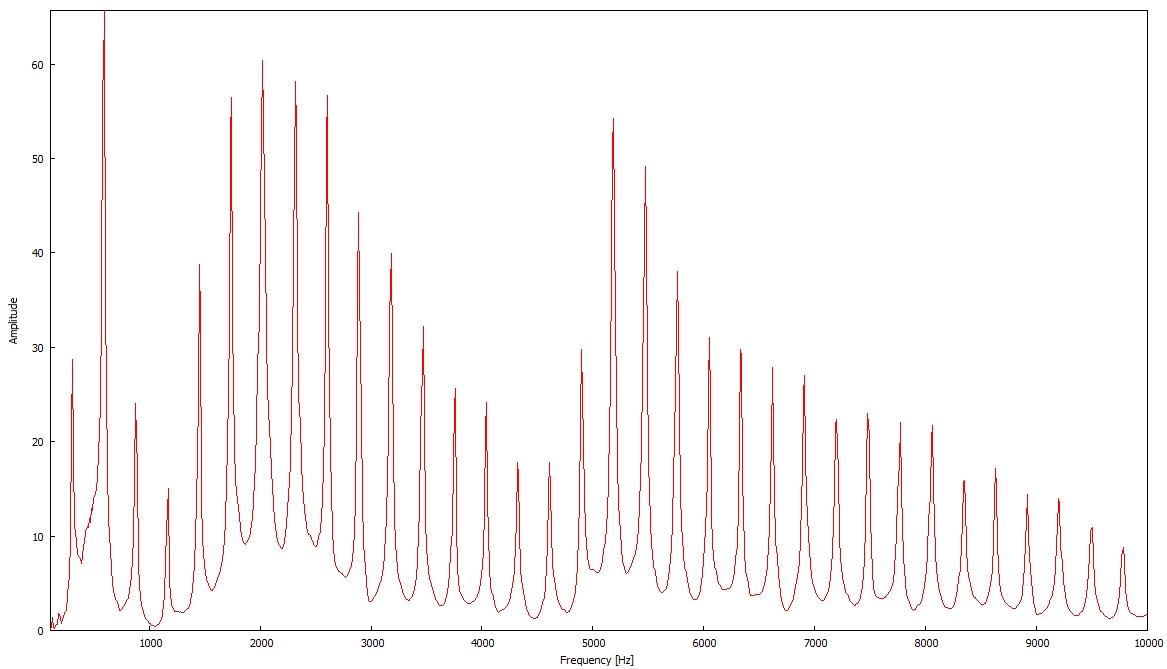
\includegraphics[width=\textwidth]{content/messungen/Chapter1/1-1img.jpg}
\caption{Übersichtsspektrum der Schallwellen in einer 600~mm langen Röhre von 0.1~kHz bis 10~kHz.}
\label{fig:1-1}
\end{figure}
Die zwei von 5~kHz bis 14~kHz aufgenommenen Spektren der 150~mm Röhre sind in den Abbildungen \ref{fig:1-2a:a} und \ref{fig:1-2b:a} dargestellt.
Zu diesen beiden Spektren sind die entsprechenden Fits in den Abbildungen \ref{fig:1-2a:b} und \ref{fig:1-2b:b} dargestellt.
Die vom Messprogramm ,,SpektrumSLC.exe'' erstellten Parameter, die die Peaks des Spektrums charakterisieren, sind in Tabelle \ref{tab:1:1} bzw. in Tabelle \ref{tab:1:2} aufgeführt.
%%%%%%%%%%%%%%%%%%%%%%%%%%
\begin{figure}
\centering
\begin{subfigure}{0.4\textwidth}
\vspace{0.8cm}
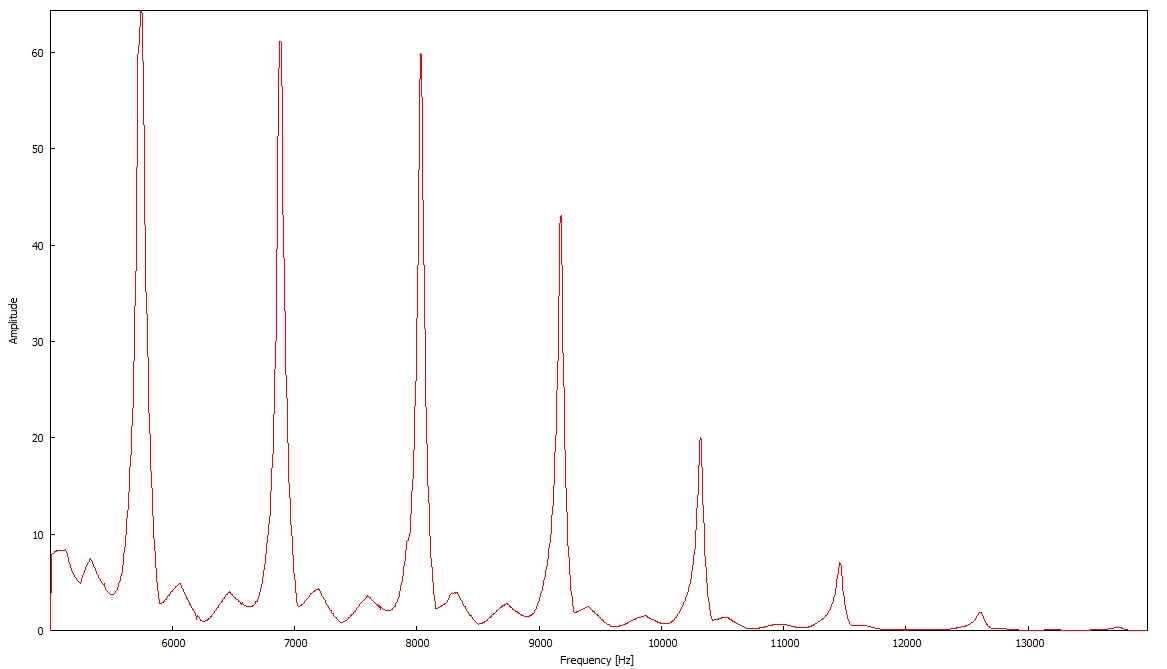
\includegraphics[width=\textwidth]{content/messungen/Chapter1/1-2img.jpg}
\subcaption{Rohdaten}
\label{fig:1-2a:a}
\end{subfigure}
\begin{subfigure}{0.4\textwidth}
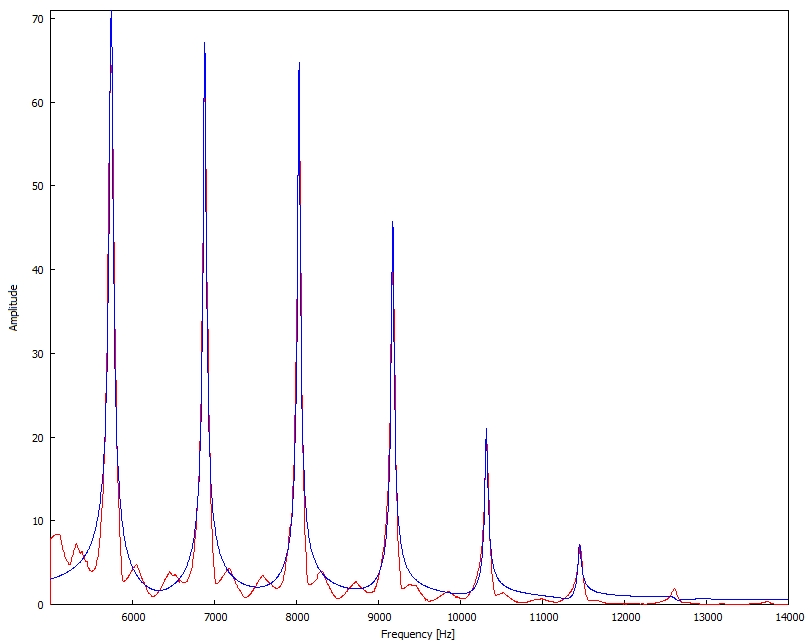
\includegraphics[width=\textwidth]{content/messungen/Chapter1/fit_img1.jpg}
\subcaption{Rohdaten mit Fit. Für Fitparameter siehe Tabelle \ref{tab:1:1}}
\label{fig:1-2a:b}
\end{subfigure}
\caption{Spektrum einer 150~mm langen Rühre von 5~kHz bis 14~kHz.}
\label{fig:1-2a}
\end{figure}
%%%%%%%%%%%%%%%%%%%%%%%%%%

%%%%%%%%%%%%%%%%%%%%%%%%%%
\begin{figure}
\centering
\begin{subfigure}{0.4\textwidth}
\vspace{0.8cm}
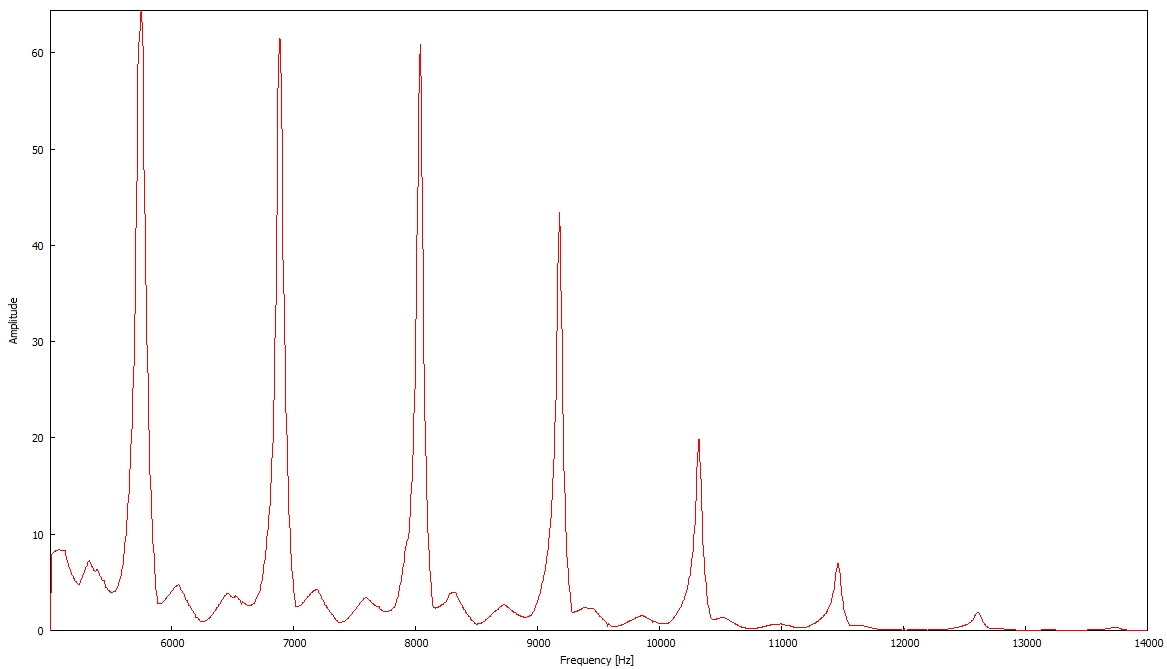
\includegraphics[width=\textwidth]{content/messungen/Chapter1/1-2-2img.jpg}
\subcaption{Rohdaten}
\label{fig:1-2b:a}
\end{subfigure}
\begin{subfigure}{0.4\textwidth}
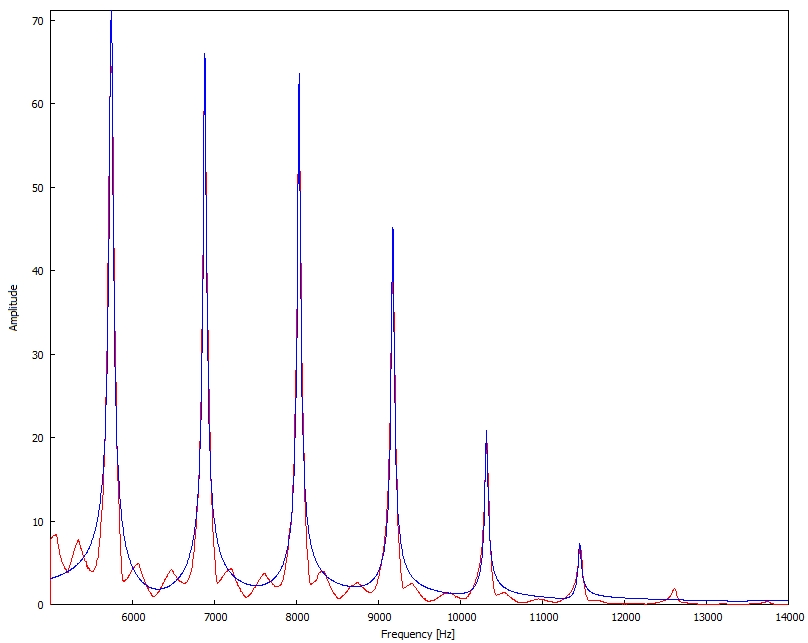
\includegraphics[width=\textwidth]{content/messungen/Chapter1/fit_img2.jpg}
\subcaption{Rohdaten mit Fit. Für Fitparameter siehe Tabelle \ref{tab:1:1}}
\label{fig:1-2b:b}
\end{subfigure}
\caption{Wiederholungsmessung des Spektrums einer 150~mm langen Rühre von 5~kHz bis 14~kHz.}
\label{fig:1-2b}
\end{figure}
%%%%%%%%%%%%%%%%%%%%%%%%%%

\begin{table}
\centering
\caption{Ergebnis des Fits aus Abbildung \ref{fig:1-2a}.}
\label{tab:1:1}
\begin{tabular}{c c c c c c c c c}
\hline
 & Peak 1 & Peak 2 & Peak 3 & Peak 4 & Peak 5 & Peak 6&Peak 7&Peak 8 \\ \hline

Frequenz in Hz& 5745.4&6885.3&8033.8&9176.0&10317&11541&126123&17242\\
Amplitude&69.9&65.8&63.5&44.6&20.0&6.45&0.41&0.20\\
Breite in Hz&21.3&16.6&14.6&15.0&16.2&20.1&52.1&4200\\
Phase in Grad&-51.0&-31.2&4.3&38.2&57.5&50.5&-140&178\\
\hline
\end{tabular}
\end{table}

\begin{table}
\centering
\caption{Ergebnis des Fits aus Abbildung \ref{fig:1-2b}.}
\label{tab:1:2}
\begin{tabular}{c c c c c c c c c}
\hline
 & Peak 1 & Peak 2 & Peak 3 & Peak 4 & Peak 5 & Peak 6&Peak 7&Peak 8 \\ \hline

Frequenz in Hz&5746.0&6886.5&8034.6&9177.1&10318&11454&13453&13665\\
Amplitude&70.0&64.8&62.0&44.1&19.9&6.60&0.02&0.18\\
Breite in Hz&21.3&17.5&15.8&15.6&16.2&18.2&512&230\\
Phase in Grad&-46.5&-26.1&9.90&51.2&72.3&72.5&-107&37.0\\
\hline
\end{tabular}
\end{table}
\FloatBarrier
\subsection{Der Kugelresonator}
\label{subsec:Der Kugelresonator}
Die Übersichtsspektren für die Winkel $\alpha=0\degree,30\degree,60\degree,90\degree,120\degree,150\degree,180\degree$ werden in den Abbildung \ref{fig:2_1_0} bis \ref{fig:2_1_180} dargestellt.
%%%%%%%%%%%%%%%%%%%%%%%%
\begin{figure}
\centering
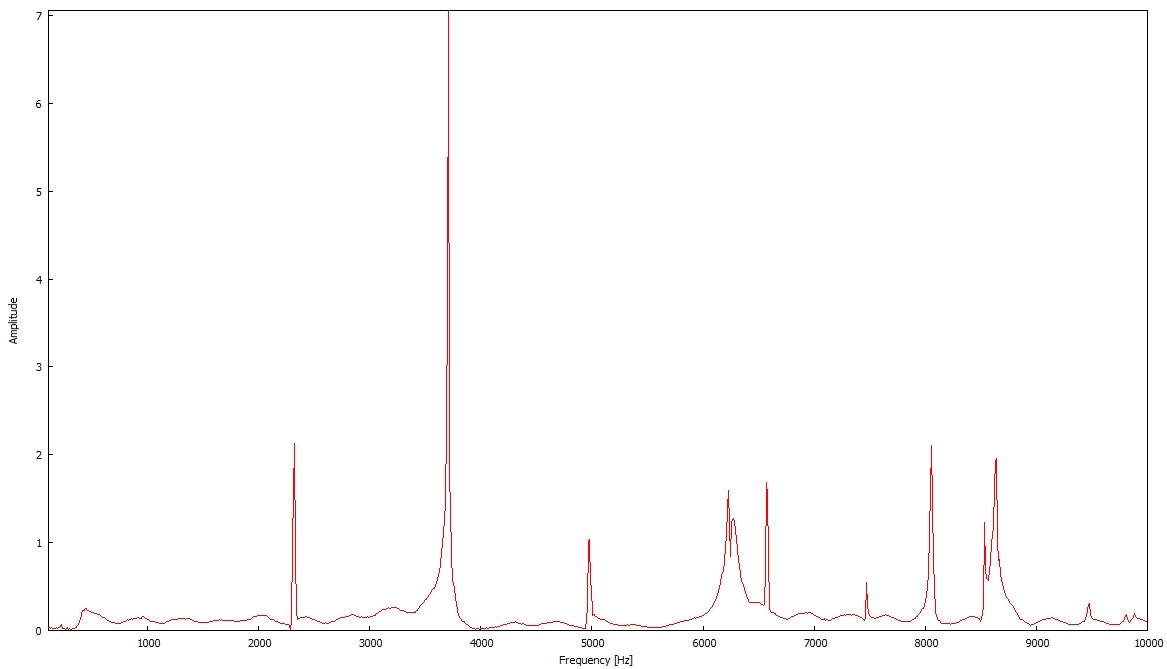
\includegraphics[width=\textwidth]{content/messungen/Chapter2new/2_1_0img.jpg}
\caption{Übersichtsspektrum des Kugelresonators von 0.1~kHz bis 10~kHz für $\alpha=0\degree$}
\label{fig:2_1_0}
\end{figure}

\begin{figure}
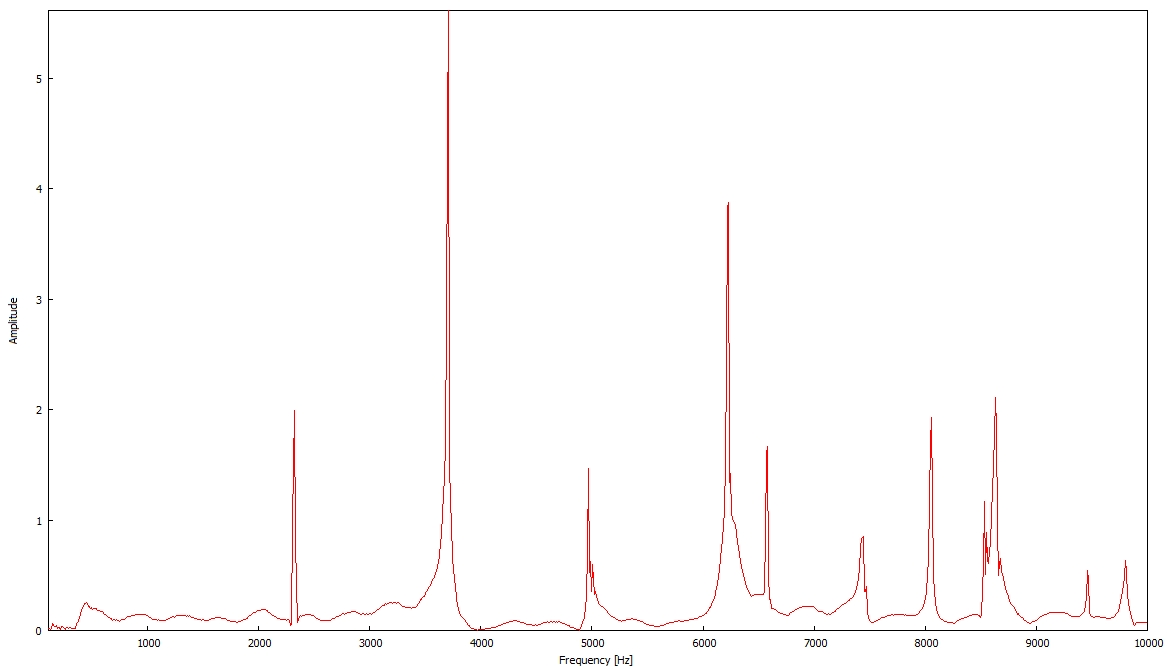
\includegraphics[width=\textwidth]{content/messungen/Chapter2new/2_1_30img.jpg}
\caption{Übersichtsspektrum des Kugelresonators von 0.1~kHz bis 10~kHz für $\alpha=30\degree$}
\label{fig:2_1_30}
\end{figure}

\begin{figure}
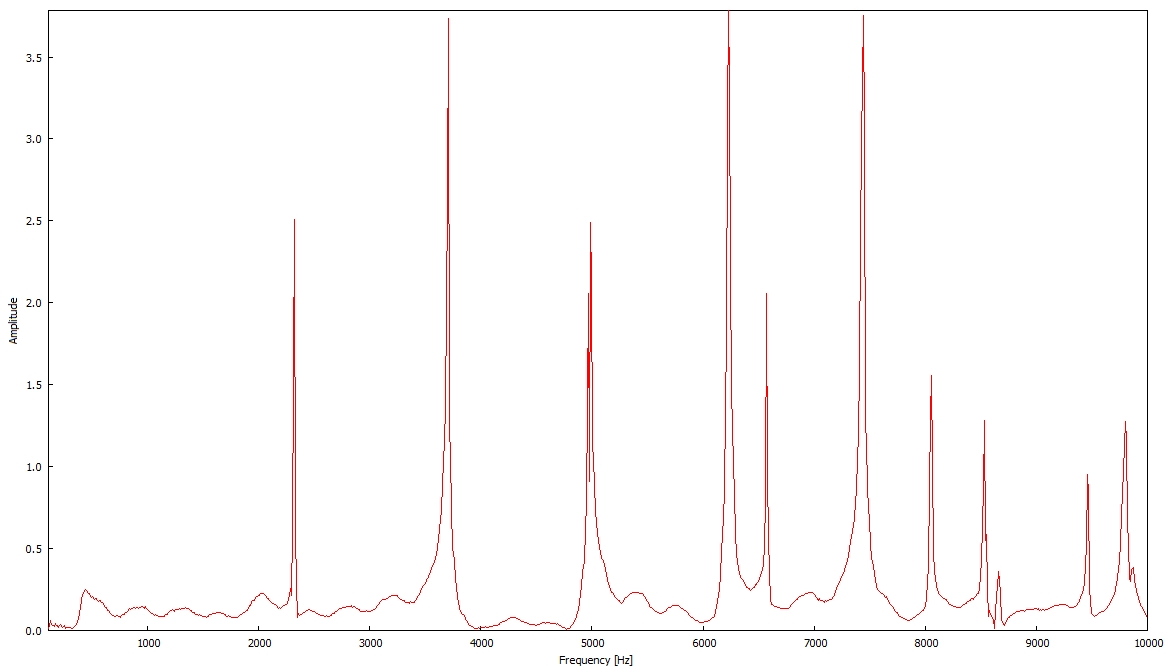
\includegraphics[width=\textwidth]{content/messungen/Chapter2new/2_1_60img.jpg}
\caption{Übersichtsspektrum des Kugelresonators von 0.1~kHz bis 10~kHz für $\alpha=60\degree$}
\label{fig:2_1_60}
\end{figure}

\begin{figure}
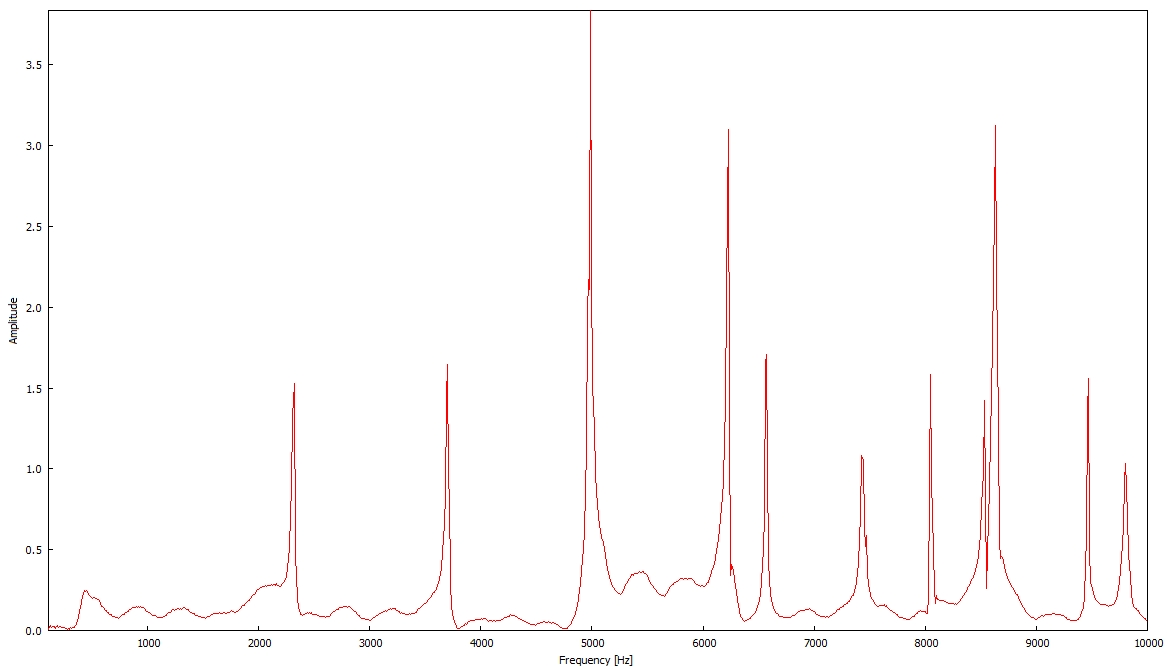
\includegraphics[width=\textwidth]{content/messungen/Chapter2new/2_1_90img.jpg}
\caption{Übersichtsspektrum des Kugelresonators von 0.1~kHz bis 10~kHz für $\alpha=90\degree$}
\label{fig:2_1_90}
\end{figure}

\begin{figure}
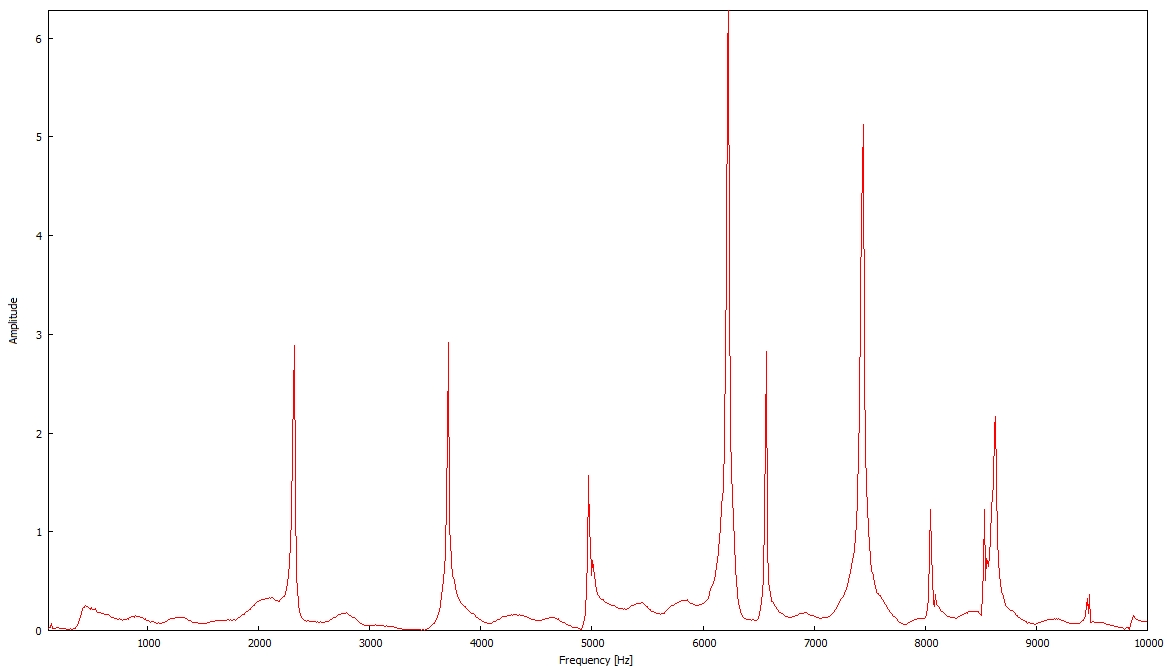
\includegraphics[width=\textwidth]{content/messungen/Chapter2new/2_1_120img.jpg}
\caption{Übersichtsspektrum des Kugelresonators von 0.1~kHz bis 10~kHz für $\alpha=120\degree$}
\label{fig:2_1_120}
\end{figure}

\begin{figure}
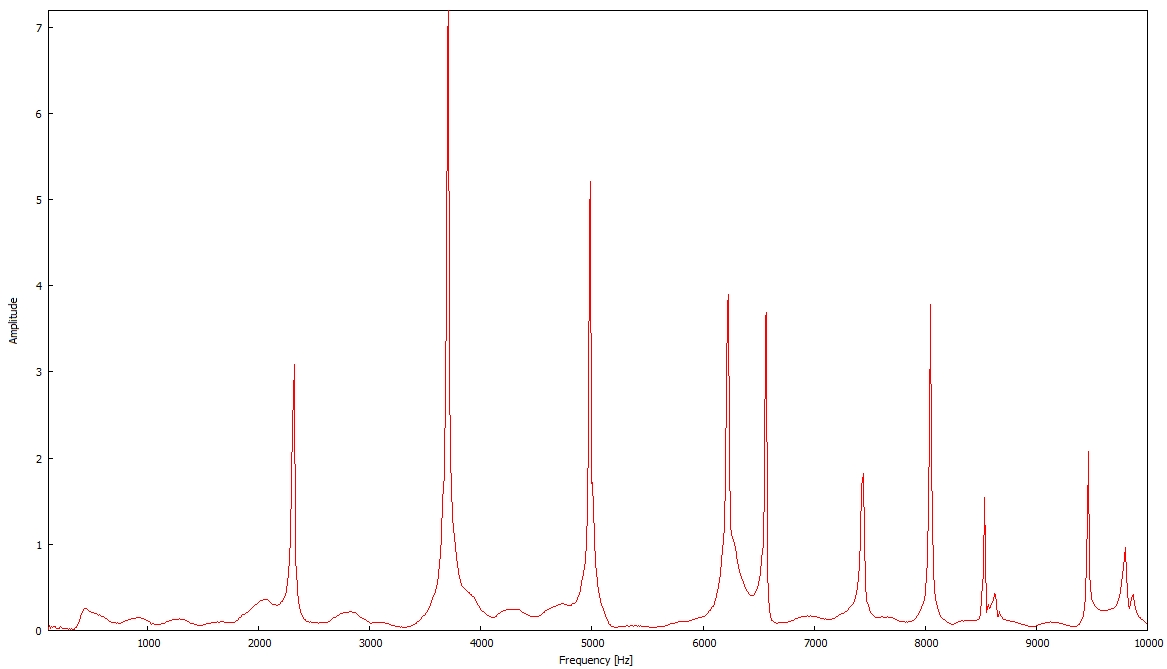
\includegraphics[width=\textwidth]{content/messungen/Chapter2new/2_1_150img.jpg}
\caption{Übersichtsspektrum des Kugelresonators von 0.1~kHz bis 10~kHz für $\alpha=150\degree$}
\label{fig:2_1_150}
\end{figure}

\begin{figure}
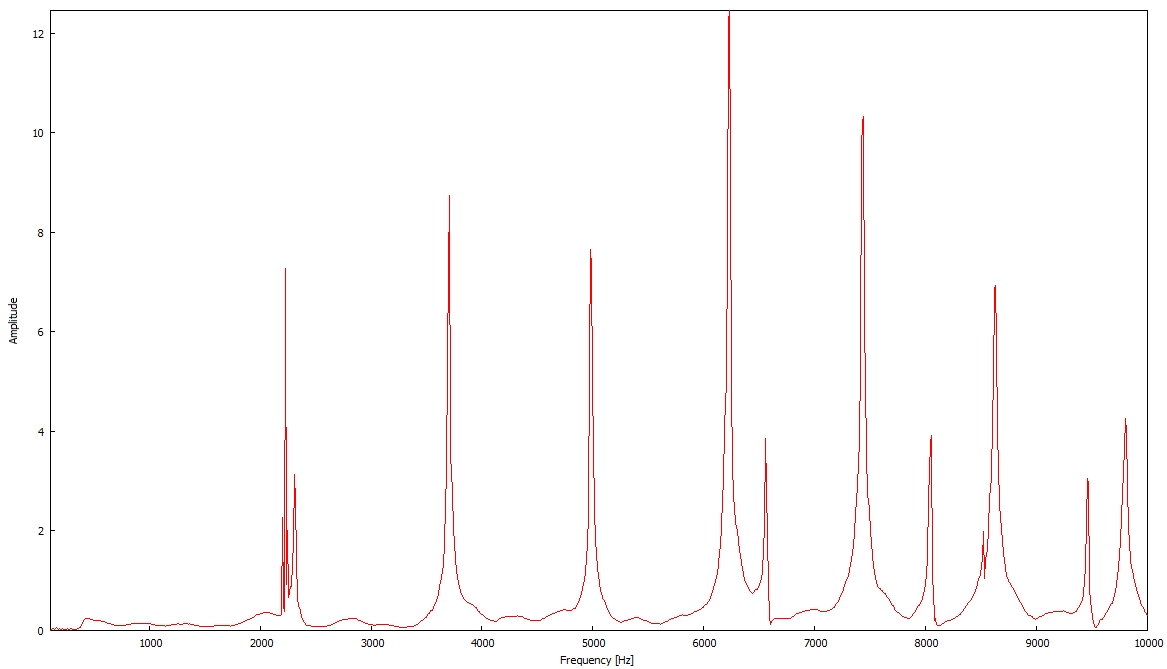
\includegraphics[width=\textwidth]{content/messungen/Chapter2new/2_1_180img.jpg}
\caption{Übersichtsspektrum des Kugelresonators von 0.1~kHz bis 10~kHz für $\alpha=180\degree$}
\label{fig:2_1_180}
\end{figure}
%%%%%%%%%%%%%%%%%%%%%%%%%%%%%
Die Abbildungen \ref{fig:2_2_0} bis \ref{fig:2_2_40} zeigen die Untersuchungsergebnisse der Resonanzstelle bei ca. 5~kHz. 
\begin{figure}
\centering
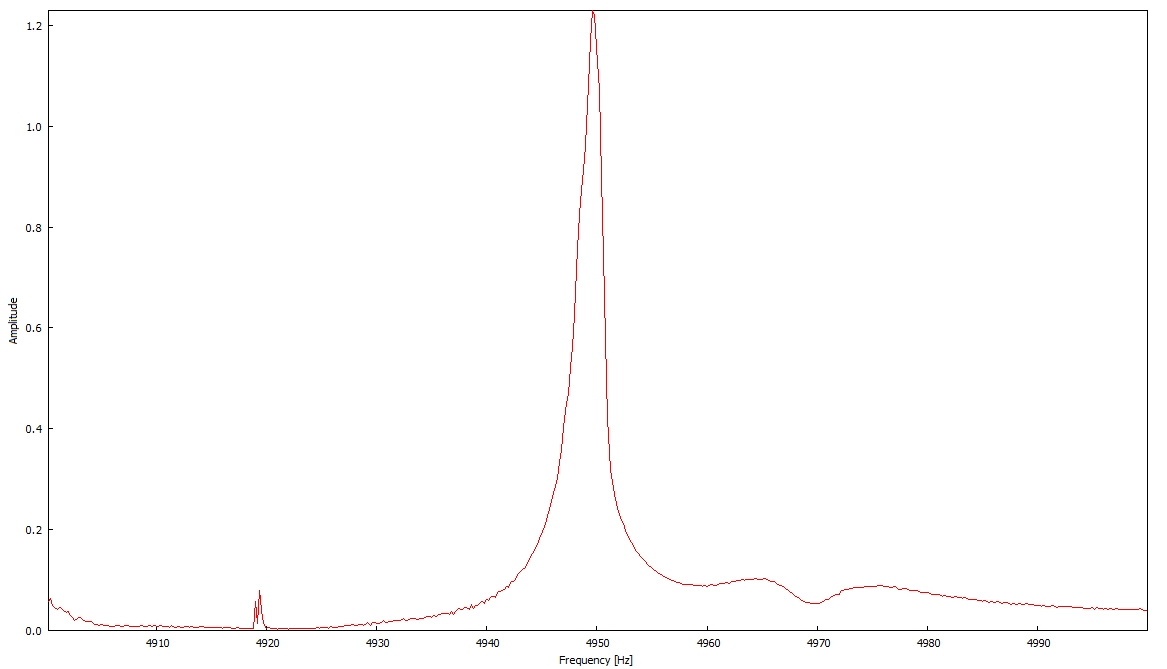
\includegraphics[width=\textwidth]{content/messungen/Chapter2new/2_2_0img.jpg}
\caption{Die dritte Resonanzstelle des Kugelresonators wird für $\alpha=0\degree$ zwischen 4.9~kHz und 5.0~kHz untersucht.}
\label{fig:2_2_0}
\end{figure}
\begin{figure}
\centering
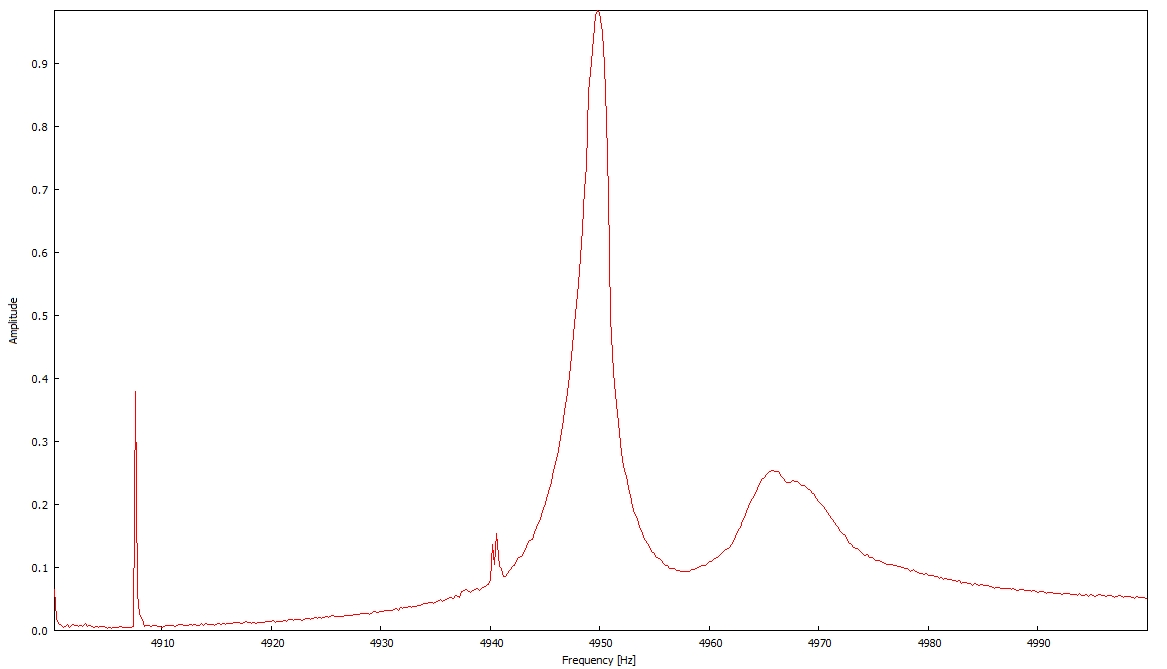
\includegraphics[width=\textwidth]{content/messungen/Chapter2new/2_2_20mg.jpg}
\caption{Die dritte Resonanzstelle des Kugelresonators wird für $\alpha=20\degree$ zwischen 4.9~kHz und 5.0~kHz untersucht.}
\label{fig:2_2_20}
\end{figure}
\begin{figure}
\centering
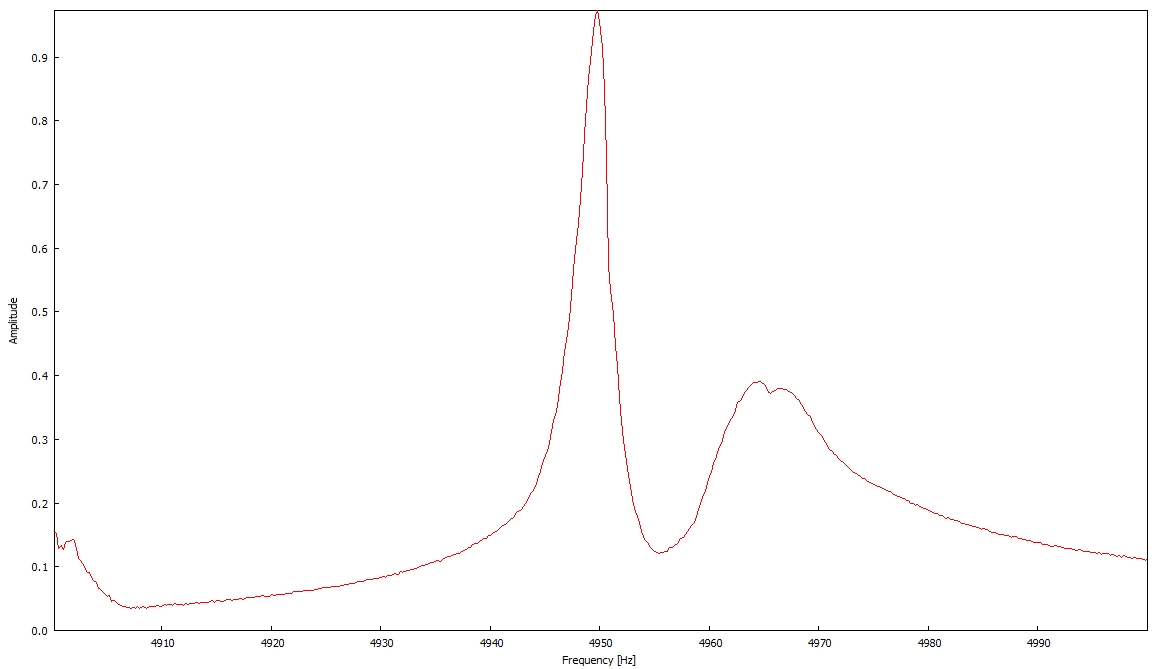
\includegraphics[width=\textwidth]{content/messungen/Chapter2new/2_2_40mg.jpg}
\caption{Die dritte Resonanzstelle des Kugelresonators wird für $\alpha=40\degree$ zwischen 4.9~kHz und 5.0~kHz untersucht.}
\label{fig:2_2_40}
\end{figure}
Um nun die Messungen an festen Resonanzstellen darzustellen wird das in Abbildung \ref{fig:2_3_180} aufgeführte von 2~kHz bis 7~kHz aufgenommene Spektrum betrachtet.
\begin{figure}
\centering
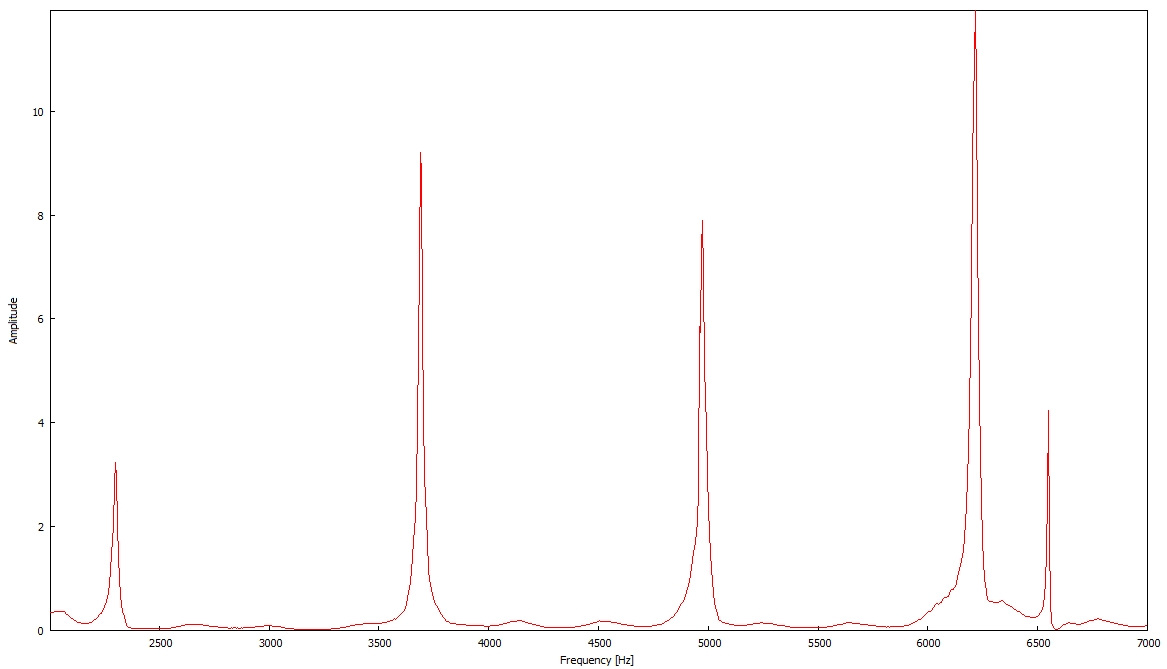
\includegraphics[width=\textwidth]{content/messungen/Chapter2new/2_3_180mg.jpg}
\caption{Spektrum des Kugelresonators von 2~kHz bis 7~kHz bei $\alpha=180\degree$.}
\label{fig:2_3_180}
\end{figure}
Die fünf zu erkennenden Resonanzstellen werden bei fester Frequenz durch variieren des Winkels $\alpha$ ausgemessen.
Es sei darauf hingewiesen, dass der Computer $\alpha$ automatisch in die gesuchte Größte $\theta$ umrechnet.
Um der Symmetrie des Kugelresonators gerecht zu werden, werden die Ergebnisse in den Polarplots \ref{fig:2_3_1} bis \ref{fig:2_3_5} dargestellt.
Die zugehörigen Messdaten sind in den Tabellen \ref{tab:2:1} bis \ref{tab:2:5} aufgeführt.
%%%%%%%%%%%%%%%%%%%%
\begin{figure}
\centering
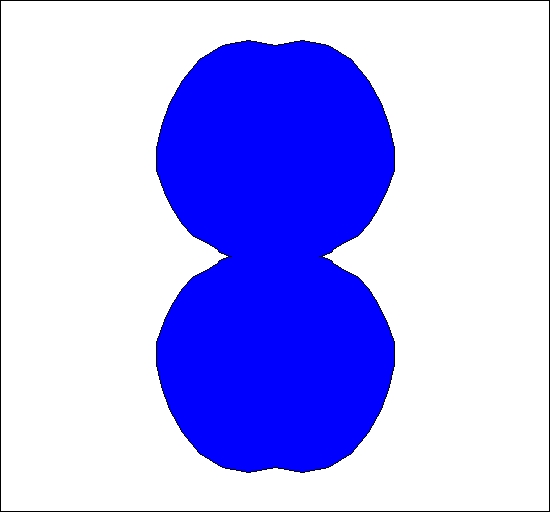
\includegraphics[width=\textwidth]{content/messungen/Chapter2new/2_3_1.jpg}
\caption{Schallamplitude in Abhängigkeit des Winkels $\theta$ bei ca. 2.30~kHz.}
\label{fig:2_3_1}
\end{figure}

\begin{figure}
\centering
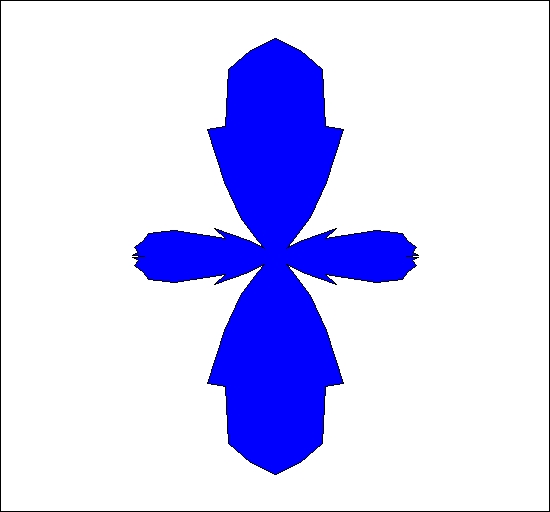
\includegraphics[width=\textwidth]{content/messungen/Chapter2new/2_3_2.jpg}
\caption{Schallamplitude in Abhängigkeit des Winkels $\theta$ bei ca. 3.69~kHz.}
\label{fig:2_3_2}
\end{figure}

\begin{figure}
\centering
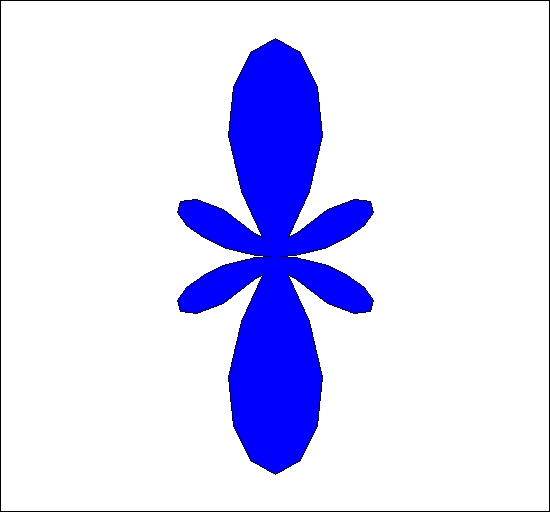
\includegraphics[width=\textwidth]{content/messungen/Chapter2new/2_3_3.jpg}
\caption{Schallamplitude in Abhängigkeit des Winkels $\theta$ bei ca. 4.98~kHz.}
\label{fig:2_3_3}
\end{figure}

\begin{figure}
\centering
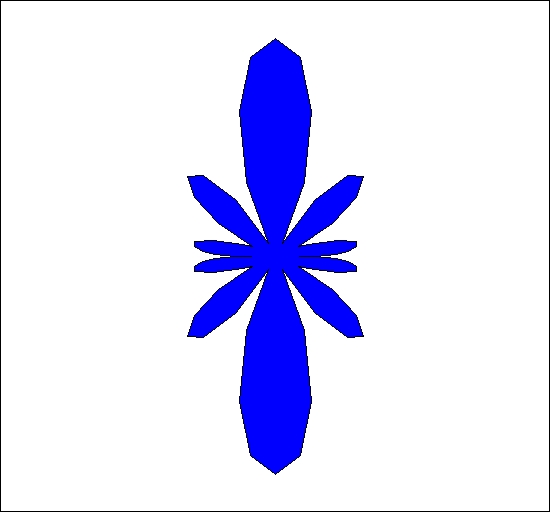
\includegraphics[width=\textwidth]{content/messungen/Chapter2new/2_3_4.jpg}
\caption{Schallamplitude in Abhängigkeit des Winkels $\theta$ bei ca. 6.21~kHze.}
\label{fig:2_3_4}
\end{figure}

\begin{figure}
\centering
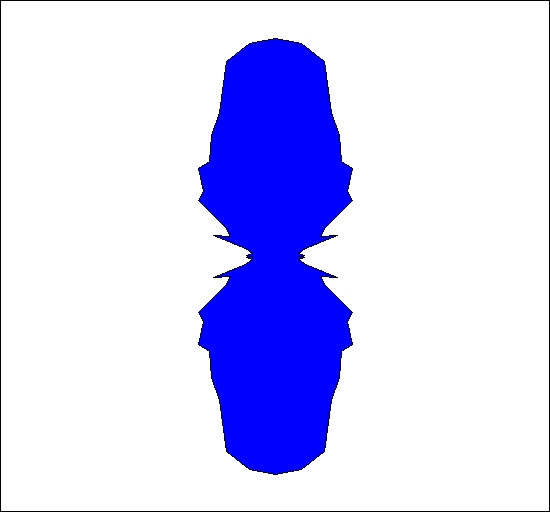
\includegraphics[width=\textwidth]{content/messungen/Chapter2new/2_3_5.jpg}
\caption{Schallamplitude in Abhängigkeit des Winkels $\theta$ bei ca. 6.55~kHz.}
\label{fig:2_3_5}
\end{figure}
%%%%%%%%%%%%%%%%%%%%%
\FloatBarrier